\chapter{Introduction}\label{chapter:introduction}

Semiconductor lasers present a very compact compact, efficient and mass producible solid state laser. They have many applications in everyday life and science, such as optical communication, data storage, printing, sensing, medical treatment, and pumping solid-state lasers.

A special type of semiconductor laser is a VECSEL (Vertical External Cavity Surface Emitting Laser). It is based on a VCSEL (Vertical Cavity Surface Emitting Laser) and emits light perpendicular to the surface of a semiconductor wafer but unlike a VCSEL, a VECSEL has an external cavity that is formed by one or more optical elements outside the wafer. This allows for more flexibility in designing the laser parameters, such as wavelength, output power, beam quality and pulse duration. VECSEL are also typically optical pumped whereas VCSEL are electrically pumped.

The basic structure of the VECSEL itself consists of an active region and a distributed Bragg reflector (DBR). Inside the active region, multiple quantum wells are located which are engineered to provide the necessary energy levels for the desired wavelength of laser emission, in this case the 2-\unit{\um} range. This wavelength range is of strong interest for many application, particularly for medical purposes and atmospheric spectroscopy. The DBR is made of alternating layers of semiconductor material with different refractive indices. By choosing the optical layer thicknesses to be one quarter of the laser wavelength, the DBR achieves high reflectivity at the desired wavelength range of the laser. 

A novel design approach incorporates a DBR for the pump wavelength as well. This new structure shows remarkable improvements in terms of efficiency and power scaling in continuous wave (CW) operation, as seen in \cref{fig:pslope}. The performance improvements in a modelocked configuration were not as significant. To get a better understanding of this, additional investigation were conducted and for this work we focused on the gain saturation characteristics.

\begin{figure}[ht]
    \centering
    \sidesubfloat[]{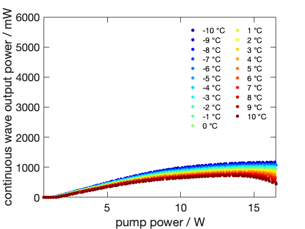
\includegraphics[width=0.46\linewidth]{images/ppwerSlope_noDBR.png}\label{fig:pslopenDBR}}
    \hfill
    \sidesubfloat[]{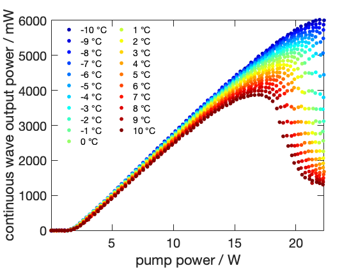
\includegraphics[width=0.46\linewidth]{images/powerSlope_DBR.png}\label{fig:pslopeDBR}}
    \caption{Continuous wave (CW) output power of a VECSEL without pump DBR a) and with pump DBR b) versus pump power under different heat sink temperature ranging from \qtyrange{-10}{10}{\celsius}. The data demonstrates the effect of the pump DBR on the power scaling performance in CW operation. The VECSEL with pump DBR shows an increase of \qty{18}{\percent} in efficiency and a sixfold increase in output power.}
    \label{fig:pslope}
\end{figure}

\section{Gain saturation}

Gain saturation describes a phenomenon that occurs when the active region of a laser is unable to maintain its gain as the pump power increases for high values. 

To study this behaviour, one measures the nonlinear behaviour of the reflectivity for an increasing amount of probe fluence, as can be seen in \cref{fig:gainSat}. To quantify this behaviour and gain some macroscopic parameters, a model based on the saturation of the absorber in a SESAM can be fitted to the data. 

\begin{equation}
    \centering
    R(F)=R_{ns} \frac{F_{sat}}{F} \ln\left\{1 + \frac{R_{ss}}{R_{ns}} \left[\exp{ \left(\frac{F}{F_{sat}}\right) } - 1\right]\right\} \exp{\left(-\frac{F}{F_2}\right)}
    \label{eq:model}
\end{equation}

The parameters from \cref{eq:model} are the saturation fluence $F_{sat}$, the small signal reflectivity $R_{ss}$, the nonsaturable reflectivity $R_{ns}$ and the roll-over parameter $F_{2}$.

The saturation fluence $F_{sat}$ is the fluence at which the reflectivity reduces to $1/e$ of its maximum. It also represents the point at which the population inversion inside the active region becomes saturated, therefore it is closely tied to the material properties of the active region.

The small signal reflectivity $R_{ss}$ refers to the reflectivity at low probe fluence, where the gain is not significantly saturated. In this regime nonlinear effects are minimal and the reflectivity can be consider the be in the linear regime and the small signal approximation can be applied and the small signal gain can be calculated as $g_{ss}=R_{ss}-100\%$.

The nonsaturable reflectivity $R_{ns}$ arises from absorption and scattering at impurities and interfaces inside the VECSEL structure. This limits the maximum performance of the VECSEL, thus reducing defect during the growing process is important. Since this effect is associated with imperfection and reflection inside the structure it remains relatively constant for different probe fluences. 

The roll-over parameter $F_2$ describes further absorption from two photon absorption or higher order effects resulting in a strong decrease in the reflectivity at high fluences.

\Cref{fig:gainSat} shows the key parameters and the fitted model with and without accounting for the roll-over for a measurement of a VECSEL with an integrated pump DBR.


\begin{figure}[ht]
    \centering
    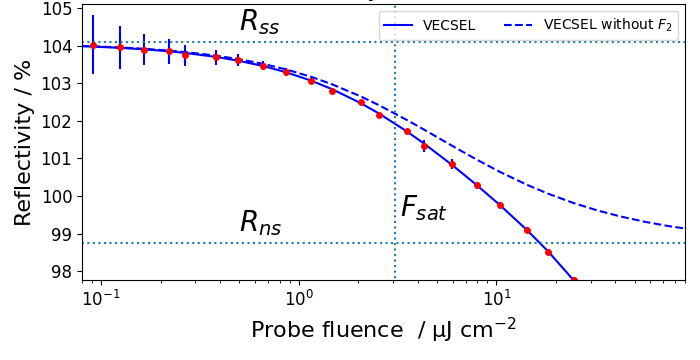
\includegraphics[width=12cm]{images/gainSat.png}
    \caption{Nonlinear reflectivity measurement for a diamond backed VECSEL with integrated pump DBR versus probe fluence. The data is shown with the fitted model utilizing \cref{eq:model} and the same model without the roll over parameter $F_2$. Additionally the different parameters $R_{ss}$, $R_{ns}$ and $F_{sat}$ are visualized.}
    \label{fig:gainSat}
\end{figure}

